%TCIDATA{LaTeXparent=0,0,relatorio.tex}



\chapter{Programas utilizados}

\section{Texto Estruturado}
\label {stsection}

\subsection{Inicialização do primeiro teste de malha aberta}
\label {stMAinit1}
\lstinputlisting{codes/init1.st}

\subsection{Inicialização do segundo teste de malha aberta}
\label {stMAinit2}
\lstinputlisting{codes/init2.st}

\subsection{Inicialização dos testes de malha fechada}
\label {stMFinit}
\lstinputlisting{codes/initP.st}

\subsection{Inicialização da rede DeviceNET}
\label{dninitST}
\lstinputlisting{codes/InitDNetST.st}

\subsection{Programa de controle em malha aberta}
\label{maprogST}
\lstinputlisting{codes/malhaAbertaT2.st}

\subsection{Programa de controle proporcional - malha fechada}
\label{mfprogST}
\lstinputlisting{codes/malhaFechadaP.st}

\section{Linguagem \textit{ladder}}
\subsection{Execução de \textit{trigger} da câmera}
\label{laddertrigger}
\begin{figure}[!ht]
\centering
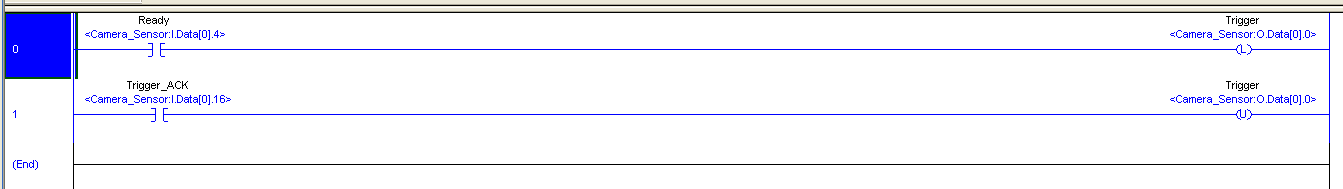
\includegraphics[width=\linewidth]{figs/ladder/camera_trigger}
\caption{\textit{Trigger} da câmera}
\end{figure}

\subsection{Rotina de parada de emergência}
\label{emergencyladder}
\begin{figure}[!ht]
\centering
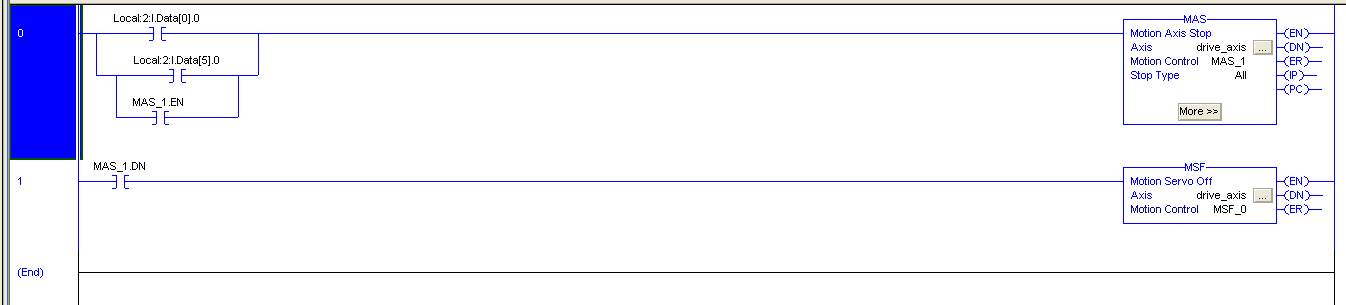
\includegraphics[width=\linewidth]{figs/ladder/parada}
\caption{Parada de emergência}
\end{figure}

\section{Programas da câmera}
\subsection{Detecção da posição horizontal da bolinha}
\label{ballhorzpos}
\begin{figure}[!ht]
\centering
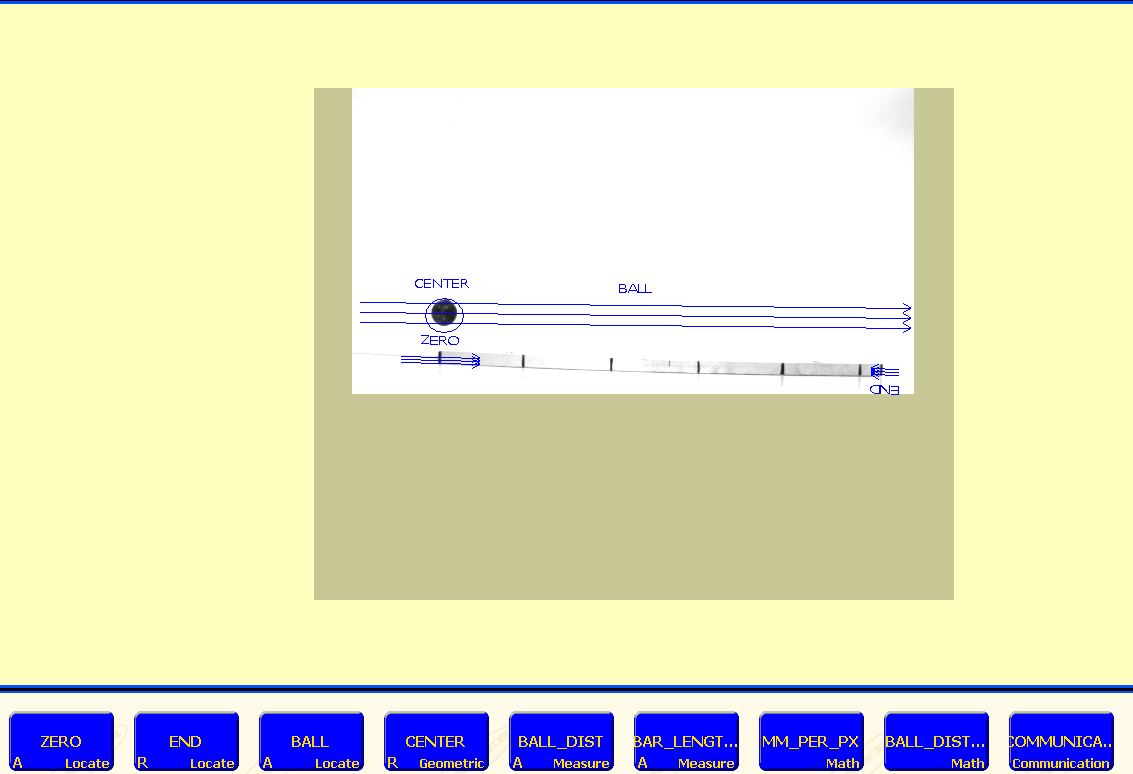
\includegraphics[width=\linewidth]{figs/presence/programaCaptura}
\caption{Detecção da posição horizontal da bolinha}
\end{figure}